\documentclass[11pt,]{article}
\usepackage{lmodern}
\usepackage{amssymb,amsmath}
\usepackage{ifxetex,ifluatex}
\usepackage{fixltx2e} % provides \textsubscript
\ifnum 0\ifxetex 1\fi\ifluatex 1\fi=0 % if pdftex
  \usepackage[T1]{fontenc}
  \usepackage[utf8]{inputenc}
\else % if luatex or xelatex
  \ifxetex
    \usepackage{mathspec}
  \else
    \usepackage{fontspec}
  \fi
  \defaultfontfeatures{Ligatures=TeX,Scale=MatchLowercase}
\fi
% use upquote if available, for straight quotes in verbatim environments
\IfFileExists{upquote.sty}{\usepackage{upquote}}{}
% use microtype if available
\IfFileExists{microtype.sty}{%
\usepackage{microtype}
\UseMicrotypeSet[protrusion]{basicmath} % disable protrusion for tt fonts
}{}
\usepackage[margin=1in]{geometry}
\usepackage{hyperref}
\hypersetup{unicode=true,
            pdftitle={How to make Beautiful Ruby Plots with Galaaz},
            pdfauthor={Rodrigo Botafogo; Daniel Mossé; University of Pittsburgh},
            pdfborder={0 0 0},
            breaklinks=true}
\urlstyle{same}  % don't use monospace font for urls
\usepackage{color}
\usepackage{fancyvrb}
\newcommand{\VerbBar}{|}
\newcommand{\VERB}{\Verb[commandchars=\\\{\}]}
\DefineVerbatimEnvironment{Highlighting}{Verbatim}{commandchars=\\\{\}}
% Add ',fontsize=\small' for more characters per line
\usepackage{framed}
\definecolor{shadecolor}{RGB}{248,248,248}
\newenvironment{Shaded}{\begin{snugshade}}{\end{snugshade}}
\newcommand{\KeywordTok}[1]{\textcolor[rgb]{0.13,0.29,0.53}{\textbf{#1}}}
\newcommand{\DataTypeTok}[1]{\textcolor[rgb]{0.13,0.29,0.53}{#1}}
\newcommand{\DecValTok}[1]{\textcolor[rgb]{0.00,0.00,0.81}{#1}}
\newcommand{\BaseNTok}[1]{\textcolor[rgb]{0.00,0.00,0.81}{#1}}
\newcommand{\FloatTok}[1]{\textcolor[rgb]{0.00,0.00,0.81}{#1}}
\newcommand{\ConstantTok}[1]{\textcolor[rgb]{0.00,0.00,0.00}{#1}}
\newcommand{\CharTok}[1]{\textcolor[rgb]{0.31,0.60,0.02}{#1}}
\newcommand{\SpecialCharTok}[1]{\textcolor[rgb]{0.00,0.00,0.00}{#1}}
\newcommand{\StringTok}[1]{\textcolor[rgb]{0.31,0.60,0.02}{#1}}
\newcommand{\VerbatimStringTok}[1]{\textcolor[rgb]{0.31,0.60,0.02}{#1}}
\newcommand{\SpecialStringTok}[1]{\textcolor[rgb]{0.31,0.60,0.02}{#1}}
\newcommand{\ImportTok}[1]{#1}
\newcommand{\CommentTok}[1]{\textcolor[rgb]{0.56,0.35,0.01}{\textit{#1}}}
\newcommand{\DocumentationTok}[1]{\textcolor[rgb]{0.56,0.35,0.01}{\textbf{\textit{#1}}}}
\newcommand{\AnnotationTok}[1]{\textcolor[rgb]{0.56,0.35,0.01}{\textbf{\textit{#1}}}}
\newcommand{\CommentVarTok}[1]{\textcolor[rgb]{0.56,0.35,0.01}{\textbf{\textit{#1}}}}
\newcommand{\OtherTok}[1]{\textcolor[rgb]{0.56,0.35,0.01}{#1}}
\newcommand{\FunctionTok}[1]{\textcolor[rgb]{0.00,0.00,0.00}{#1}}
\newcommand{\VariableTok}[1]{\textcolor[rgb]{0.00,0.00,0.00}{#1}}
\newcommand{\ControlFlowTok}[1]{\textcolor[rgb]{0.13,0.29,0.53}{\textbf{#1}}}
\newcommand{\OperatorTok}[1]{\textcolor[rgb]{0.81,0.36,0.00}{\textbf{#1}}}
\newcommand{\BuiltInTok}[1]{#1}
\newcommand{\ExtensionTok}[1]{#1}
\newcommand{\PreprocessorTok}[1]{\textcolor[rgb]{0.56,0.35,0.01}{\textit{#1}}}
\newcommand{\AttributeTok}[1]{\textcolor[rgb]{0.77,0.63,0.00}{#1}}
\newcommand{\RegionMarkerTok}[1]{#1}
\newcommand{\InformationTok}[1]{\textcolor[rgb]{0.56,0.35,0.01}{\textbf{\textit{#1}}}}
\newcommand{\WarningTok}[1]{\textcolor[rgb]{0.56,0.35,0.01}{\textbf{\textit{#1}}}}
\newcommand{\AlertTok}[1]{\textcolor[rgb]{0.94,0.16,0.16}{#1}}
\newcommand{\ErrorTok}[1]{\textcolor[rgb]{0.64,0.00,0.00}{\textbf{#1}}}
\newcommand{\NormalTok}[1]{#1}
\usepackage{graphicx,grffile}
\makeatletter
\def\maxwidth{\ifdim\Gin@nat@width>\linewidth\linewidth\else\Gin@nat@width\fi}
\def\maxheight{\ifdim\Gin@nat@height>\textheight\textheight\else\Gin@nat@height\fi}
\makeatother
% Scale images if necessary, so that they will not overflow the page
% margins by default, and it is still possible to overwrite the defaults
% using explicit options in \includegraphics[width, height, ...]{}
\setkeys{Gin}{width=\maxwidth,height=\maxheight,keepaspectratio}
\IfFileExists{parskip.sty}{%
\usepackage{parskip}
}{% else
\setlength{\parindent}{0pt}
\setlength{\parskip}{6pt plus 2pt minus 1pt}
}
\setlength{\emergencystretch}{3em}  % prevent overfull lines
\providecommand{\tightlist}{%
  \setlength{\itemsep}{0pt}\setlength{\parskip}{0pt}}
\setcounter{secnumdepth}{5}
% Redefines (sub)paragraphs to behave more like sections
\ifx\paragraph\undefined\else
\let\oldparagraph\paragraph
\renewcommand{\paragraph}[1]{\oldparagraph{#1}\mbox{}}
\fi
\ifx\subparagraph\undefined\else
\let\oldsubparagraph\subparagraph
\renewcommand{\subparagraph}[1]{\oldsubparagraph{#1}\mbox{}}
\fi

%%% Use protect on footnotes to avoid problems with footnotes in titles
\let\rmarkdownfootnote\footnote%
\def\footnote{\protect\rmarkdownfootnote}

%%% Change title format to be more compact
\usepackage{titling}

% Create subtitle command for use in maketitle
\newcommand{\subtitle}[1]{
  \posttitle{
    \begin{center}\large#1\end{center}
    }
}

\setlength{\droptitle}{-2em}

  \title{How to make Beautiful Ruby Plots with Galaaz}
    \pretitle{\vspace{\droptitle}\centering\huge}
  \posttitle{\par}
    \author{Rodrigo Botafogo \\ Daniel Mossé \\ University of Pittsburgh}
    \preauthor{\centering\large\emph}
  \postauthor{\par}
      \predate{\centering\large\emph}
  \postdate{\par}
    \date{November 19th, 2018}

% usar portugues do Brasil
% \usepackage[brazilian]{babel}
\usepackage[utf8]{inputenc}

\usepackage{geometry}
\geometry{a4paper, top=1in}

% needed for kableExtra
\usepackage{longtable}
\usepackage{multirow}
\usepackage[table]{xcolor}
\usepackage{wrapfig}
\usepackage{float}
\usepackage{colortbl}
\usepackage{pdflscape}
\usepackage{tabu}
\usepackage{threeparttable}
\usepackage[normalem]{ulem}

\usepackage{bbm}
\usepackage{booktabs}
\usepackage{expex}

\usepackage{graphicx}

\usepackage{fancyhdr}
% set the header and foot style
% style 'fancy' adds the section name on the header
% and the page number on the footer
\pagestyle{fancy}

% style 'fancyhf' leaves header and footer empty
%\fancyhf{}

% sets the left head element to \rightmark, which contains the
% current section (\leftmark is the current chapter)
%\fancyhead[L]{\rightmark} .

% sets the right head element to the page number.
% \fancyhead[R]{\thepage}

% lets the head rule disappear.
% \renewcommand{\headrulewidth}{0pt}
% Possible selectors for the optional argument of \fancyhead/\fancyfoot
% are L (left), C (center) or R (right) for the position of the element
% and E (even) or O (odd) to distinguish even and odd pages. If you omit
% E/O the element is set for all pages.

% \usepackage{lipsum}

% make available command lastpage
\usepackage{lastpage}

% default fontsize 11pt better to add
% fontsize on the yaml header
% \usepackage[fontsize=11pt]{scrextend}

% comandos para formatar uma tabela
\usepackage{array}
\newcolumntype{L}[1]{>{\raggedright\let\newline\\\arraybackslash\hspace{0pt}}m{#1}}
\newcolumntype{C}[1]{>{\centering\let\newline\\\arraybackslash\hspace{0pt}}m{#1}}
\newcolumntype{R}[1]{>{\raggedleft\let\newline\\\arraybackslash\hspace{0pt}}m{#1}}

% necessário if we need to import other latex documents
\usepackage{import}

% Command to import an R variable to latex
\newcommand{\RtoLatex}[2]{\newcommand{#1}{#2}}

% 
%\newcommand{\atraso}[1]{\color{red} \textbf {Tempo desde a Assinatura do Contrato: #1 dias}}

\begin{document}
\maketitle

{
\setcounter{tocdepth}{2}
\tableofcontents
}
\section{Introduction}\label{introduction}

According to Wikipedia ``Ruby is a dynamic, interpreted, reflective,
object-oriented, general-purpose programming language. It was designed
and developed in the mid-1990s by Yukihiro''Matz" Matsumoto in Japan."
It reached high popularity with the development of Ruby on Rails (RoR)
by David Heinemeier Hansson. RoR is a web application framework first
released around 2005. It makes extensive use of Ruby's metaprogramming
features. With RoR, Ruby became very popular. According to
\href{https://www.tiobe.com/tiobe-index/ruby/}{Ruby's Tiobe index} it
peeked in popularity around 2008. Then it's popularity declined until
2015 when it started picking up again. At the time of this writing
(November 2018), the Tiobe index puts ruby in 16th position.

Python, a similar language to Ruby, ranks 4th in the index. Java, C and
C++ take the first three positions. Ruby is often criticized for its
focus on web applications. But Ruby can do
\href{https://github.com/markets/awesome-ruby}{much more} than just web
applications. Yet, for scientific computing, Ruby lags way behind Python
and R. Python has Django framework for web, NumPy for numerical arrays,
Pandas for data analysis. R is a free software environment for
statistical computing and graphics with thousands of libraries for data
analysis.

Until recently, there was no real perspective for Ruby to bridge this
gap. Implementing a complete scientific computing infrastructure would
take too long. Comes GraalVM into the picture:

\begin{quote}
GraalVM is a universal virtual machine for running applications written
in JavaScript, Python 3, Ruby, R, JVM-based languages like Java, Scala,
Kotlin, and LLVM-based languages such as C and C++.

GraalVM removes the isolation between programming languages and enables
interoperability in a shared runtime. It can run either standalone or in
the context of OpenJDK, Node.js, Oracle Database, or MySQL.

GraalVM allows you to write polyglot applications with a seamless way to
pass values from one language to another. With GraalVM there is no
copying or marshaling necessary as it is with other polyglot systems.
This lets you achieve high performance when language boundaries are
crossed. Most of the time there is no additional cost for crossing a
language boundary at all.

Often developers have to make uncomfortable compromises that require
them to rewrite their software in other languages. For example:

\begin{itemize}
\tightlist
\item
  That library is not available in my language. I need to rewrite it.
\item
  That language would be the perfect fit for my problem, but we cannot
  run it in our environment.
\item
  That problem is already solved in my language, but the language is too
  slow.
\end{itemize}

With GraalVM we aim to allow developers to freely choose the right
language for the task at hand without making compromises.
\end{quote}

As stated above, GraalVM is a \emph{universal} virtual machine that
allows Ruby and R (and other languages) to run on the same environment.
GraalVM allows polyglot applications to \emph{seamlessly} interact with
one another and pass values from one language to the other. Galaaz, a
gem for Ruby, intends to tightly couple Ruby and R and allow those
languages to interact in a way that the user will be unaware of such
interaction.

Library wrapping is an usual way of bringing features from one language
into another. To improve performance, Python often wraps more efficient
C libraries. For the Python developer, the existence of such C libraries
is of no concern. The problem with library wrapping is that for any new
library, there is the need to handcraft a new wrapper.

Galaaz, instead of wrapping a single C or R library, wraps the whole of
the R language in Ruby. Doing so, all thousands of R libraries are
available to Ruby developers. Also any new library developed in R will
be available without a new wrapping effort.

This article shows how Ruby can use R's ggplot2 library tranparantly,
and bring to Ruby the power of high quality scientific plotting. it also
shows that migrating from R to Ruby with Galaaz is a matter of small
syntactic changes. Using Ruby, the R developer can use all of Ruby's
powerful OO features. It also becomes much easier to move code from the
analysis phase to the production phase.

In this article we will explore the R ToothGrowth dataset. In doing so,
we will create some boxplots. A primer on boxplot is available in
\href{https://towardsdatascience.com/understanding-boxplots-5e2df7bcbd51}{this
article}.

We will also create a Corporate Template ensuring that plots will have a
consistent visualization. This template is build using a Ruby module.
There is a way of building ggplot themes that will work the same as the
Ruby module. Yet, writing a new theme requires specific knowledge. Ruby
modules are standard to the language and don't need special knowledge.

In
\href{https://towardsdatascience.com/ruby-plotting-with-galaaz-an-example-of-tightly-coupling-ruby-and-r-in-graalvm-520b69e21021}{this
blog} we show a scatter plot in Ruby also with Galaaz.

\section{gKnit}\label{gknit}

\emph{Knitr} is an application that converts text written in rmarkdown
to many different output formats. For instance, a writer can convert an
rmarkdown document to HTML, \(LaTex\), docx and many other formats.
Rmarkdown documents can contain text and \emph{code chunks}. Knitr
formats code chunks in a grayed box in the output document. It also
executes the code chunks and formats the output in a white box. Every
line of output from the execution code is preceded by `\#\#'.

Knitr allows code chunks to be in R, Python, Ruby and dozens of other
languages. Yet, while R and Python chunks can share data, in other
languages, chunks are independent. This means that a variable defined in
one chunk cannot be used in another chunk.

With \emph{gKnit} Ruby code chunks can share data. In gKnit each Ruby
chunk executes in its own scope and thus, local variable defined in a
chunk are not accessible by other chunks. Yet, All chunks execute in the
scope of a `chunk' class and instance variables (`@'), are available in
all chunks.

\section{Exploring the Dataset}\label{exploring-the-dataset}

Let's start by exploring our selected dataset. ToothGrowth is an R
dataset. A dataset is like an excel spreadsheet, but in which each
column has only one type of data. For instance one column can have
float, the other integer, and a third strings. This dataset analyses the
length of odontoblasts (cells responsible for tooth growth) in 60 guinea
pigs, where each animal received one of three dose levels of Vitamin C
(0.5, 1, and 2 mg/day) by one of two delivery methods, orange juice (OJ)
or ascorbic acid (a form of vitamin C and coded as VC).

The ToothGrowth dataset contains three columns: `len', `supp' and
`dose'. Let's take a look at a few rows of this dataset. In Galaaz, to
have access to an R variable we use the corresponding Ruby symbol
preceeded by the tilda (`\textasciitilde{}') function. Note in the
following chunk that Ruby's `@tooth\_growth' is assigned the value of
`\textasciitilde{}:ToothGrowth'. `ToothGrowth' is the R variable
containing the dataset of interest.

\begin{Shaded}
\begin{Highlighting}[]
\CommentTok{# Read the R ToothGrowth variable and assign it to the}
\CommentTok{# Ruby instance variable @tooth_growth that will be }
\CommentTok{# available to all Ruby chunks in this document.}
\OtherTok{@tooth_growth}\NormalTok{ = ~}\StringTok{:ToothGrowth}
\CommentTok{# print the first few elements of the dataset}
\NormalTok{puts }\OtherTok{@tooth_growth}\NormalTok{.head}
\end{Highlighting}
\end{Shaded}

\begin{verbatim}
##    len supp dose
## 1  4.2   VC  0.5
## 2 11.5   VC  0.5
## 3  7.3   VC  0.5
## 4  5.8   VC  0.5
## 5  6.4   VC  0.5
## 6 10.0   VC  0.5
\end{verbatim}

Great! We've managed to read the ToothGrowth dataset and take a look at
its elements. We see here the first 6 rows of the dataset. To access a
column, follow the dataset name with a dot (`.') and the name of the
column. Also use dot notation to chain methods in usual Ruby style.

\begin{Shaded}
\begin{Highlighting}[]
\CommentTok{# Access the tooth_growth 'len' column and print the first few}
\CommentTok{# elements of this column with the 'head' method.}
\NormalTok{puts }\OtherTok{@tooth_growth}\NormalTok{.len.head}
\end{Highlighting}
\end{Shaded}

\begin{verbatim}
## [1]  4.2 11.5  7.3  5.8  6.4 10.0
\end{verbatim}

The `dose' column contains a numeric value wiht either, 0.5, 1 or 2.
Although those are number, they are better interpreted as a
\href{https://swcarpentry.github.io/r-novice-inflammation/12-supp-factors/}{factor
or cathegory}. So, let's convert our `dose' column from numeric to
`factor'. In R, the function `as.factor' is used to convert data in a
vector to factors. To use this function from Galaaz the dot (`.') in the
function name is substituted by '\_\_`(double underline). The function
'as.factor' becomes 'R.as\_\_factor' or just 'as\_\_factor' when
chaining.

\begin{Shaded}
\begin{Highlighting}[]
\CommentTok{# convert the dose to a factor}
\OtherTok{@tooth_growth}\NormalTok{.dose = }\OtherTok{@tooth_growth}\NormalTok{.dose.as__factor}
\end{Highlighting}
\end{Shaded}

Let's explore some more details of this dataset. In particular, let's
look at its dimensions, structure and summary statistics.

\begin{Shaded}
\begin{Highlighting}[]
\NormalTok{puts }\OtherTok{@tooth_growth}\NormalTok{.dim}
\end{Highlighting}
\end{Shaded}

\begin{verbatim}
## [1] 60  3
\end{verbatim}

This dataset has 60 rows, one for each subject and 3 columns, as we have
already seen.

Note that we do not call `puts' when using the `str' function. This
functions does not return anything and prints the structure of the
dataset as a side effect.

\begin{Shaded}
\begin{Highlighting}[]
\OtherTok{@tooth_growth}\NormalTok{.str}
\end{Highlighting}
\end{Shaded}

\begin{verbatim}
## 'data.frame':    60 obs. of  3 variables:
##  $ len : num  4.2 11.5 7.3 5.8 6.4 10 11.2 11.2 5.2 7 ...
##  $ supp: Factor w/ 2 levels "OJ","VC": 2 2 2 2 2 2 2 2 2 2 ...
##  $ dose: Factor w/ 3 levels "0.5","1","2": 1 1 1 1 1 1 1 1 1 1 ...
\end{verbatim}

Observe that both variables `supp' and `dose' are factors. The system
made variable `supp' a factor automatically, since it contais two
strings OJ and VC.

Finally, using the summary method, we get the statistical summary for
the dataset

\begin{Shaded}
\begin{Highlighting}[]
\NormalTok{puts }\OtherTok{@tooth_growth}\NormalTok{.summary}
\end{Highlighting}
\end{Shaded}

\begin{verbatim}
##       len        supp     dose   
##  Min.   : 4.20   OJ:30   0.5:20  
##  1st Qu.:13.07   VC:30   1  :20  
##  Median :19.25           2  :20  
##  Mean   :18.81                   
##  3rd Qu.:25.27                   
##  Max.   :33.90
\end{verbatim}

\section{Doing the Data Analysis}\label{doing-the-data-analysis}

\subsection{Quick plot for seing the
data}\label{quick-plot-for-seing-the-data}

Let's now create our first plot with the given data by accessing ggplot2
from Ruby. For Rubyist that have never seen or used ggplot2, here is the
description of ggplot found on its home page:

\begin{quote}
``ggplot2 is a system for declaratively creating graphics, based on
\emph{The Grammar of Graphics}. You provide the data, tell ggplot2 how
to map variables to aesthetics, what graphical primitives to use, and it
takes care of the details.''
\end{quote}

This description might be a bit cryptic and it is best to see it at work
to understand it. Basically, in the \emph{grammar of graphics}
developers add layers of components such as grid, axis, data, title,
subtitle and also graphical primitives such as \emph{bar plot},
\emph{box plot}, to form the final graphics.

In order to make a plot, we use the `ggplot' function to the dataset. In
R, this would be written as
\texttt{ggplot(\textless{}dataset\textgreater{},\ ...)}. In Galaaz, use
either \texttt{R.ggplot(\textless{}dataset\textgreater{},\ ...)}, or
\texttt{\textless{}dataset\textgreater{}.ggplot(...)}. In the graph
specification bellow, we use the second notation that looks more Ruby
like. The plot specifies the `dose' on the \(x\) axis and the `length'
on the \(y\) axis with the `aes' method. `E.aes(x: :dose, y: :len)'. To
specify the type of plot to create add a geom to the plot. For a
boxplot, the geom is R.geom\_boxplot.

Note also that we have a call to `R.png' before plotting and
'R.dev\_\_off' after the print statement. `R.png' opens a `png' device
for outputting the plot. 'R.dev\_\_off' closes the device and creates
the `png' file. If we do no pass a name to the `png' function, the image
gets a default name of `Rplot\textless{}nnn\textgreater{}' where
\textless{}nnn\textgreater{} is the number of the plot. We can then
include the generated `png' file in the document by adding an rmarkdown
directive.

\begin{Shaded}
\begin{Highlighting}[]
\NormalTok{require }\StringTok{'ggplot'}

\NormalTok{R.png(}\StringTok{"figures/dose_len.png"}\NormalTok{)}

\NormalTok{e = }\OtherTok{@tooth_growth}\NormalTok{.ggplot(E.aes(}\StringTok{x: :dose}\NormalTok{, }\StringTok{y: :len}\NormalTok{))}
\NormalTok{print e + R.geom_boxplot}

\NormalTok{R.dev__off}
\end{Highlighting}
\end{Shaded}

\begin{figure}
\centering
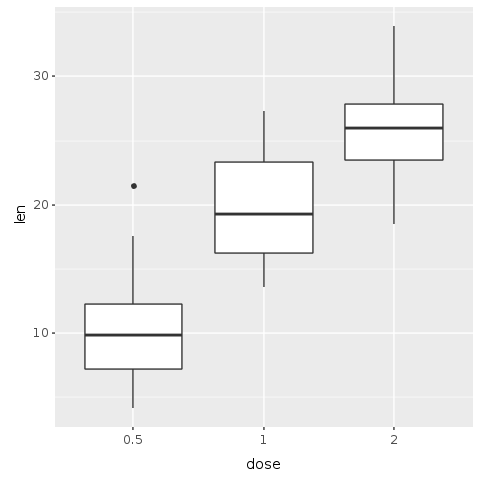
\includegraphics[width=0.70000\textwidth]{figures/dose_len.png}
\caption{}
\end{figure}

Great! We've just managed to create and save our first plot in Ruby with
only four lines of code. We can see with this plot a clear trend: as the
dose of the supplement is increased, so is the length of teeth.

\subsection{Facetting the plot}\label{facetting-the-plot}

This first plot shows a trend, but our data has information about two
different forms of delivery method, either by Orange Juice (OJ) or by
Vitamin C (VC). Let's then try to create a plot that explicits the
effect of each delivery method. This next plot is a \emph{facetted} plot
where each delivery method gets is own plot. On the left side, the plot
shows the OJ delivery method. On the right side, we see the VC delivery
method. To obtain this plot, we use the `R.facet\_grid' function, that
automatically creates the facets based on the delivery method factors.
The parameter to the `facet\_grid' method is a
\href{https://thomasleeper.com/Rcourse/Tutorials/formulae.html}{\emph{formula}}.

In Galaaz, formulas are written a bit differently than in R. The
following changes are necessary:

\begin{itemize}
\tightlist
\item
  R symbols are represented by the same Ruby symbol prefixed with the
  `+' method. The symbol \texttt{x} in R becomes \texttt{+:x} in Ruby;
\item
  The `\textasciitilde{}' operator in R becomes `=\textasciitilde{}' in
  Ruby. The formula \texttt{x\ \textasciitilde{}\ y} in R is written as
  \texttt{+:x\ =\textasciitilde{}\ +:y} in Ruby;
\item
  The `.' symbol in R becomes `+:all'
\end{itemize}

Another way of writing a formula is to use the `formula' function with
the actual formula as a string. The formula
\texttt{x\ \textasciitilde{}\ y} in R can be written as
\texttt{R.formula("x\ \textasciitilde{}\ y")}. For more complex
formulas, the use of the `formula' function is preferred.

The formula \texttt{+:all\ =\textasciitilde{}\ +:supp} indicates to the
`facet\_grid' function that it needs to facet the plot based on the
\texttt{supp} variable and split the plot vertically. Changing the
formula to \texttt{+:supp\ =\textasciitilde{}\ +:all} would split the
plot horizontally.

\begin{Shaded}
\begin{Highlighting}[]
\NormalTok{R.png(}\StringTok{"figures/facet_by_delivery.png"}\NormalTok{)}

\OtherTok{@base_tooth}\NormalTok{ = }\OtherTok{@tooth_growth}\NormalTok{.ggplot(E.aes(}\StringTok{x: :dose}\NormalTok{, }\StringTok{y: :len}\NormalTok{, }\StringTok{group: :dose}\NormalTok{))}

\OtherTok{@bp}\NormalTok{ = }\OtherTok{@base_tooth}\NormalTok{ + R.geom_boxplot +}
      \CommentTok{# Split in vertical direction}
\NormalTok{      R.facet_grid(+}\StringTok{:all}\NormalTok{ =~ +}\StringTok{:supp}\NormalTok{)}
      
\NormalTok{puts }\OtherTok{@bp}

\NormalTok{R.dev__off}
\end{Highlighting}
\end{Shaded}

\begin{figure}
\centering
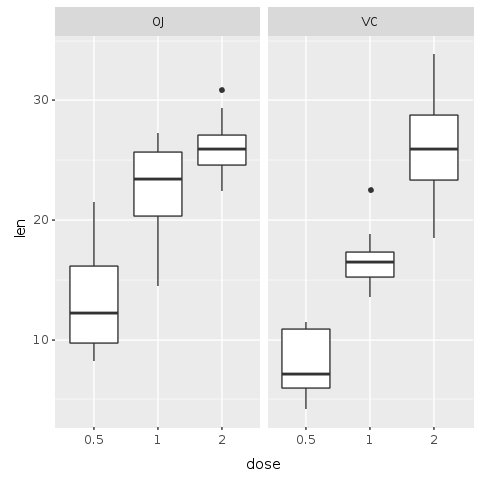
\includegraphics[width=0.70000\textwidth]{figures/facet_by_delivery.png}
\caption{}
\end{figure}

It now becomes clear that although both methods of delivery have a
direct impact on tooth growth, method (OJ) is non-linear having a higher
impact with smaller doses of ascorbic acid and reducing it's impact as
the dose increases. With the (VC) approach, the impact seems to be more
linear.

\subsection{Adding Color}\label{adding-color}

If this paper was about data analysis, we should make a better analysis
of the trends and should improve the statistical analysis. But we are
interested in working with ggplot in Ruby. So, Let's add some color to
this plot to make the trend and comparison more visible. In the
following plot, the boxes are color coded by dose. To add color, it is
enough to add \texttt{fill:\ :dose} to the aesthetic of boxplot. With
this command each `dose' factor gets its own color.

\begin{Shaded}
\begin{Highlighting}[]
\NormalTok{R.png(}\StringTok{"figures/facets_by_delivery_color.png"}\NormalTok{)}

\OtherTok{@bp}\NormalTok{ = }\OtherTok{@bp}\NormalTok{ + R.geom_boxplot(E.aes(}\StringTok{fill: :dose}\NormalTok{))}
\NormalTok{puts }\OtherTok{@bp}

\NormalTok{R.dev__off}
\end{Highlighting}
\end{Shaded}

\begin{figure}
\centering
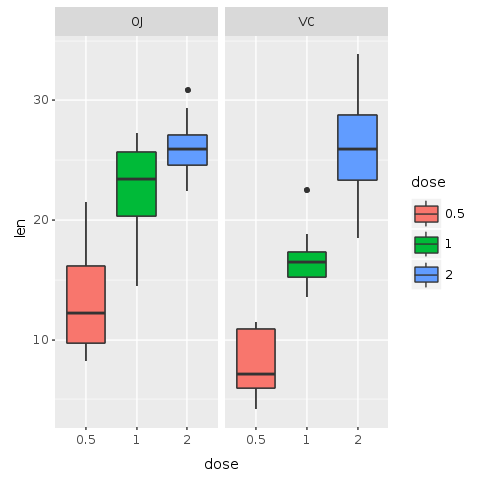
\includegraphics[width=0.70000\textwidth]{figures/facets_by_delivery_color.png}
\caption{}
\end{figure}

Facetting helps us compare the general trends in the (OJ) and (VC)
delivery methods. Adding color allow us to compare specifically how each
dosage impacts the teeth growth. It is possible to observe that with
smaller doses, up to 1mg, (OJ) performs better than (VC) (red color).
For 2mg, both (OJ) and (VC) have the same median, but (OJ) is less
disperse (blue color). For 1mg (green color), (OJ) is significantly
bettern than (VC). By this very quick analysis, it seems that (OJ) is a
better delivery method than (VC).

\subsection{Clarifying the data}\label{clarifying-the-data}

Boxplots give us a nice idea of the distribution of data, but looking at
those plots with large colored boxes leaves us wondering what is going
on on those boxes. According to Edward Tufte in Envisioning Information:

\begin{quote}
Thin data rightly prompts suspicions: ``What are they leaving out? Is
that really everything they know? What are they hiding? Is that all they
did?'' Now and then it is claimed that vacant space is ``friendly''
(anthropomorphizing an inherently murky idea) but \emph{it is not how
much empty space there is, but rather how it is used. It is not how much
information there is, but rather how effectively it is arranged.}
\end{quote}

And he states:

\begin{quote}
A most unconventional design strategy is revealed: \emph{to clarify, add
detail.}
\end{quote}

Let's then use this wisdom and add yet another layer of data to our
plot, so that we clarify it with detail and do not leave large empty
boxes. In this next plot, we add data points for each of the 60 pigs in
the experiment. For that, add the function `R.geom\_point' to the plot.

\begin{Shaded}
\begin{Highlighting}[]
\NormalTok{R.png(}\StringTok{"figures/facets_with_points.png"}\NormalTok{)}

\CommentTok{# Split in vertical direction}
\OtherTok{@bp}\NormalTok{ = }\OtherTok{@bp}\NormalTok{ + R.geom_point}

\NormalTok{puts }\OtherTok{@bp}

\NormalTok{R.dev__off}
\end{Highlighting}
\end{Shaded}

\begin{figure}
\centering
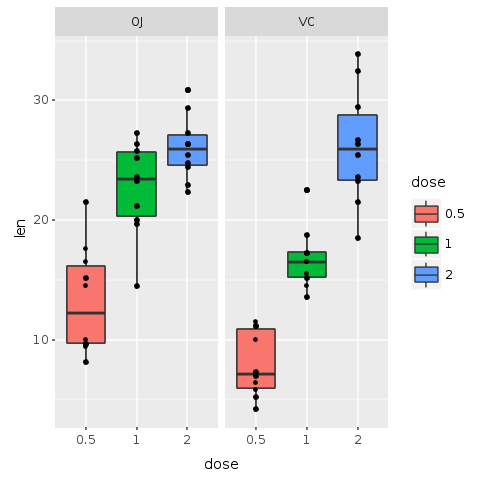
\includegraphics[width=0.70000\textwidth]{figures/facets_with_points.png}
\caption{}
\end{figure}

Now we can see the actual distribution of all the 60 subject. Actually,
this is not totally true. We have a hard time seing all 60 subjects. It
seems that some points might be placed one over the other hiding useful
information.

But no sweat! Another layer might solve the problem. In the following
plot a new layer called `geom\_jitter' is added to the plot. This adds
randomness to the position of the points, making it easier to see all of
then and preventing data hiding. We also add color and change the shape
of the points, making them even easier to see.

\begin{Shaded}
\begin{Highlighting}[]
\NormalTok{R.png(}\StringTok{"figures/facets_with_jitter.png"}\NormalTok{)}

\CommentTok{# Split in vertical direction}
\NormalTok{puts }\OtherTok{@bp}\NormalTok{ + R.geom_jitter(}\StringTok{shape: }\DecValTok{23}\NormalTok{, }\StringTok{color: "cyan3"}\NormalTok{, }\StringTok{size: }\DecValTok{1}\NormalTok{)}

\NormalTok{R.dev__off}
\end{Highlighting}
\end{Shaded}

\begin{figure}
\centering
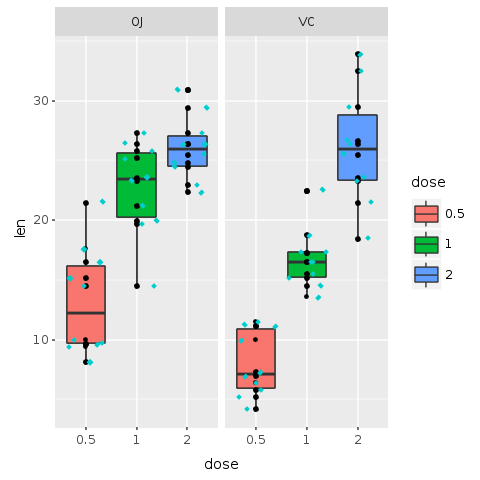
\includegraphics[width=0.70000\textwidth]{figures/facets_with_jitter.png}
\caption{}
\end{figure}

Now we can see all 60 points in the graph. We have here a much higher
information density and we can see outliers and subjects distribution.

\section{Preparing the Plot for
Presentation}\label{preparing-the-plot-for-presentation}

We have come a long way since our first plot. As was already said, this
is not an article about data analysis and the focus is on the
integration of Ruby and ggplot. So, let's assume that the analysis is
now done. Yet, ending the analysis does not mean that the work is done.
On the contrary, the hardest part is yet to come!

After the analysis it is necessary to communicate it by making a final
plot for presentation. The last plot has all the information we want to
share, but it is not very pleasing to the eye.

\subsection{Improving Colors}\label{improving-colors}

Let's start by trying to improve colors. For now, we will not use the
jitter layer. The previous plot has three bright colors that have no
relashionship between them. Is there any obvious, or non-obvious for
that matter, interpretation for the colors? Clearly, they are just
random colors selected automatically by our software. Although those
colors helped us understand the data, for a final presentation random
colors can distract the viewer.

In the following plot we use shades function `scale\_fill\_manual' to
change the colors of the boxes and order of labels. For colors we use
shades of blue for each dosage, with light blue (`cyan') representing
the lower dose and deep blue (`deepskyblue4') the higher dose. Also the
smaller value (0.5) is on the botton of the labels and (2) at the top.
This ordering seems more natural and matches with the actual order of
the colors in the plot.

\begin{Shaded}
\begin{Highlighting}[]
\NormalTok{R.png(}\StringTok{"figures/facets_by_delivery_color2.png"}\NormalTok{)}

\OtherTok{@bp}\NormalTok{ = }\OtherTok{@bp}\NormalTok{ +}
\NormalTok{      R.scale_fill_manual(}\StringTok{values: }\NormalTok{R.c(}\StringTok{"cyan"}\NormalTok{, }\StringTok{"deepskyblue"}\NormalTok{, }\StringTok{"deepskyblue4"}\NormalTok{),}
                          \StringTok{breaks: }\NormalTok{R.c(}\StringTok{"2"}\NormalTok{,}\StringTok{"1"}\NormalTok{,}\StringTok{"0.5"}\NormalTok{))}

\NormalTok{puts }\OtherTok{@bp}

\NormalTok{R.dev__off}
\end{Highlighting}
\end{Shaded}

\begin{figure}
\centering
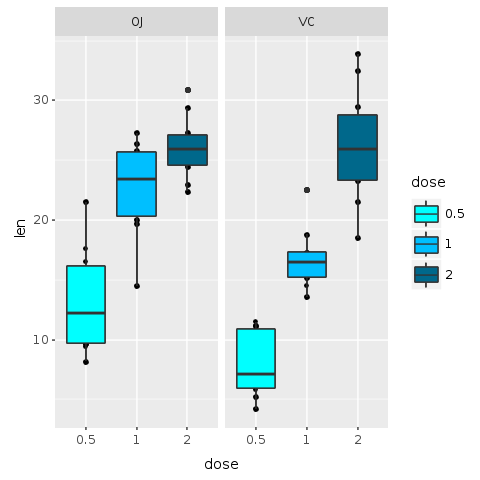
\includegraphics[width=0.70000\textwidth]{figures/facets_by_delivery_color2.png}
\caption{}
\end{figure}

\subsection{Violin Plot and Jitter}\label{violin-plot-and-jitter}

The boxplot with jitter did look a bit overwhelming. The next plot uses
a variation of a boxplot known as a \emph{violin plot} with jittered
data.

\href{https://en.wikipedia.org/wiki/Violin_plot}{From Wikipedia}

\begin{quote}
A violin plot is a method of plotting numeric data. It is similar to a
box plot with a rotated kernel density plot on each side.

A violin plot has four layers. The outer shape represents all possible
results, with thickness indicating how common. (Thus the thickest
section represents the mode average.) The next layer inside represents
the values that occur 95\% of the time. The next layer (if it exists)
inside represents the values that occur 50\% of the time. The central
dot represents the median average value.
\end{quote}

\begin{Shaded}
\begin{Highlighting}[]
\NormalTok{R.png(}\StringTok{"figures/violin_with_jitter.png"}\NormalTok{)}

\OtherTok{@violin}\NormalTok{ = }\OtherTok{@base_tooth}\NormalTok{ + R.geom_violin(E.aes(}\StringTok{fill: :dose}\NormalTok{)) + }
\NormalTok{   R.facet_grid(+}\StringTok{:all}\NormalTok{ =~ +}\StringTok{:supp}\NormalTok{) +}
\NormalTok{   R.geom_jitter(}\StringTok{shape: }\DecValTok{23}\NormalTok{, }\StringTok{color: "cyan3"}\NormalTok{, }\StringTok{size: }\DecValTok{1}\NormalTok{) +}
\NormalTok{   R.scale_fill_manual(}\StringTok{values: }\NormalTok{R.c(}\StringTok{"cyan"}\NormalTok{, }\StringTok{"deepskyblue"}\NormalTok{, }\StringTok{"deepskyblue4"}\NormalTok{),}
                       \StringTok{breaks: }\NormalTok{R.c(}\StringTok{"2"}\NormalTok{,}\StringTok{"1"}\NormalTok{,}\StringTok{"0.5"}\NormalTok{))}

\NormalTok{puts }\OtherTok{@violin}

\NormalTok{R.dev__off}
\end{Highlighting}
\end{Shaded}

\begin{figure}
\centering
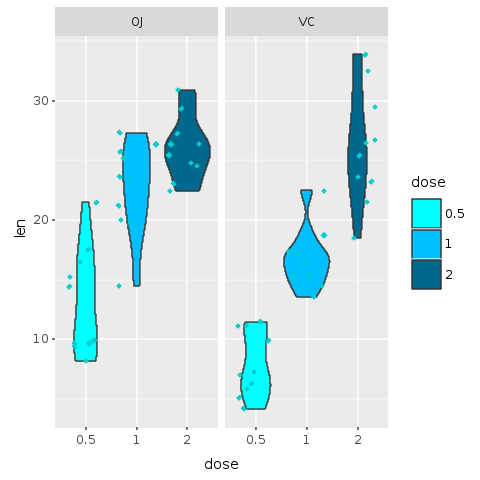
\includegraphics[width=0.70000\textwidth]{figures/violin_with_jitter.png}
\caption{}
\end{figure}

This plot is an alternative to the original boxplot. For the final
presentation, it is important to think which graphics will be best
understood by our audience. A violin plot is a less known plot and could
add mental overhead, yet, in my opinion, it does look a lit bit better
than the boxplot and provides even more information than the boxplot
with jitter.

\subsection{Adding Decoration}\label{adding-decoration}

Our final plot is starting to take shape, but a presentation plot should
have at least a title, labels on the axis and maybe some other
decorations. Let's start adding those. Since decoration requires more
graph area, this new plot has a `width' and `height' specification. When
there is no specification, the default values for width and height are
480.

The `labs' function adds require decoration. In this example we use
`title', `subtitle', `x' for the \(x\) axis label and `y', for the \(y\)
axis label, and `caption' for information about the plot.

\begin{Shaded}
\begin{Highlighting}[]
\NormalTok{R.png(}\StringTok{"figures/facets_with_decorations.png"}\NormalTok{, }\StringTok{width: }\DecValTok{540}\NormalTok{, }\StringTok{height: }\DecValTok{560}\NormalTok{)}

\NormalTok{caption = <<-}\KeywordTok{EOT}
\OtherTok{Length of odontoblasts in 60 guinea pigs. }
\OtherTok{Each animal received one of three dose levels of vitamin C.}
\KeywordTok{EOT}

\OtherTok{@decorations}\NormalTok{ =}
\NormalTok{  R.labs(}\StringTok{title: "Tooth Growth:  Length by Dose"}\NormalTok{,}
         \StringTok{subtitle: "Faceted by delivery method, (OJ) or (VC)"}\NormalTok{,}
         \StringTok{x: "Dose (mg)"}\NormalTok{, }\StringTok{y: "Teeth length"}\NormalTok{,}
         \StringTok{caption: }\NormalTok{caption)}

\NormalTok{puts }\OtherTok{@bp}\NormalTok{ + }\OtherTok{@decorations}

\NormalTok{R.dev__off}
\end{Highlighting}
\end{Shaded}

\begin{figure}
\centering
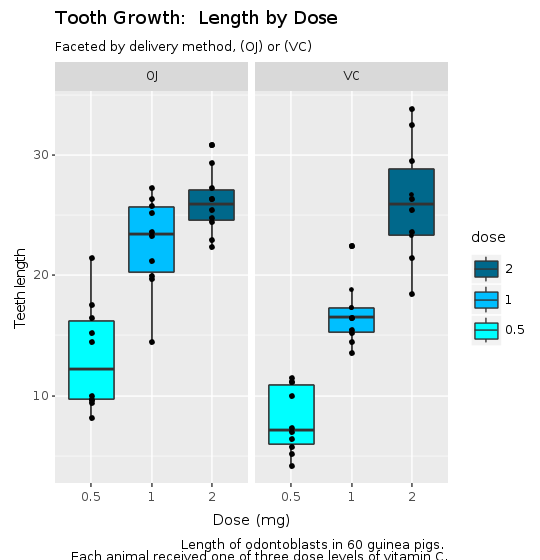
\includegraphics[width=0.70000\textwidth]{figures/facets_with_decorations.png}
\caption{}
\end{figure}

\subsection{The Corp Theme}\label{the-corp-theme}

We are almost done. But the plot does not yet look nice to the eye. We
are still distracted by many aspects of the graph. First, the back font
color does not look good. Then plot background, borders, grids all add
clutter to the plot.

We will now define our corporate theme. In this theme, we remove borders
and grids. The background if left for faceted plots but removed for
non-faceted plots. Font colors are a shade o blue (color: `\#00080').
Axis labels are moved near the end of the axis and written in `bold'.

\begin{Shaded}
\begin{Highlighting}[]
\KeywordTok{module} \DataTypeTok{CorpTheme}

\NormalTok{  R.install_and_loads }\StringTok{'RColorBrewer'}
  
  \CommentTok{#---------------------------------------------------------------------------------}
  \CommentTok{# face can be  (1=plain, 2=bold, 3=italic, 4=bold-italic)}
  \CommentTok{#---------------------------------------------------------------------------------}
  
  \KeywordTok{def} \DecValTok{self}\NormalTok{.text_element(size, }\StringTok{face: "plain"}\NormalTok{, }\StringTok{hjust: }\DecValTok{nil}\NormalTok{)}
\NormalTok{    E.element_text(}\StringTok{color: "#000080"}\NormalTok{, }
                   \StringTok{face: }\NormalTok{face,}
                   \StringTok{size: }\NormalTok{size,}
           \StringTok{hjust: }\NormalTok{hjust)}
  \KeywordTok{end}
  
  \CommentTok{#---------------------------------------------------------------------------------}
  \CommentTok{# Defines the plot theme (visualization).  In this theme we remove major and minor}
  \CommentTok{# grids, borders and background.  We also turn-off scientific notation.}
  \CommentTok{#---------------------------------------------------------------------------------}
  
  \KeywordTok{def} \DecValTok{self}\NormalTok{.global_theme(faceted = }\DecValTok{false}\NormalTok{)}
    
\NormalTok{    R.options(}\StringTok{scipen: }\DecValTok{999}\NormalTok{)  }\CommentTok{# turn-off scientific notation like 1e+48}
    \CommentTok{#    R.theme_set(R.theme_bw)}
    
    \CommentTok{# remove major grids}
\NormalTok{    gb = R.theme(}\StringTok{panel__grid__major: }\NormalTok{E.element_blank())}
    \CommentTok{# remove minor grids}
\NormalTok{    gb = gb + R.theme(}\StringTok{panel__grid__minor: }\NormalTok{E.element_blank)}
    \CommentTok{# gb = R.theme(panel__grid__minor: E.element_blank)}
    \CommentTok{# remove border}
\NormalTok{    gb = gb + R.theme(}\StringTok{panel__border: }\NormalTok{E.element_blank)}
    \CommentTok{# remove background. When working with faceted graphs, the background makes}
    \CommentTok{# it easier to see each facet, so leave it}
\NormalTok{    gb = gb + R.theme(}\StringTok{panel__background: }\NormalTok{E.element_blank) }\KeywordTok{if}\NormalTok{ !faceted}
    \CommentTok{# Change axis font}
\NormalTok{    gb = gb + R.theme(}\StringTok{axis__text: }\NormalTok{text_element(}\DecValTok{8}\NormalTok{))}
    \CommentTok{# change axis title font}
\NormalTok{    gb = gb + R.theme(}\StringTok{axis__title: }\NormalTok{text_element(}\DecValTok{10}\NormalTok{, }\StringTok{face: "bold"}\NormalTok{, }\StringTok{hjust: }\DecValTok{1}\NormalTok{))}
    \CommentTok{# change font of title}
\NormalTok{    gb = gb + R.theme(}\StringTok{title: }\NormalTok{text_element(}\DecValTok{12}\NormalTok{, }\StringTok{face: "bold"}\NormalTok{))}
    \CommentTok{# change font of subtitle}
\NormalTok{    gb = gb + R.theme(}\StringTok{plot__subtitle: }\NormalTok{text_element(}\DecValTok{9}\NormalTok{))}
    \CommentTok{# change font of captions}
\NormalTok{    gb = gb + R.theme(}\StringTok{plot__caption: }\NormalTok{text_element(}\DecValTok{8}\NormalTok{))}

  \KeywordTok{end}
   
\KeywordTok{end}
\end{Highlighting}
\end{Shaded}

\subsection{Final Box Plot}\label{final-box-plot}

Here is our final boxplot, without jitter.

\begin{Shaded}
\begin{Highlighting}[]
\NormalTok{R.png(}\StringTok{"figures/final_box_plot.png"}\NormalTok{, }\StringTok{width: }\DecValTok{540}\NormalTok{, }\StringTok{height: }\DecValTok{560}\NormalTok{)}

\NormalTok{puts }\OtherTok{@bp}\NormalTok{ + }\OtherTok{@decorations}\NormalTok{ + }\DataTypeTok{CorpTheme}\NormalTok{.global_theme(}\StringTok{faceted: }\DecValTok{true}\NormalTok{)}

\NormalTok{R.dev__off}
\end{Highlighting}
\end{Shaded}

\begin{figure}
\centering
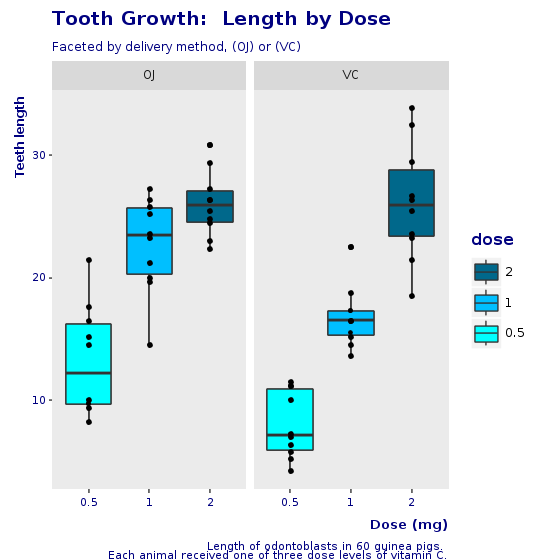
\includegraphics[width=0.70000\textwidth]{figures/final_box_plot.png}
\caption{}
\end{figure}

\subsection{Final Violin Plot}\label{final-violin-plot}

Here is the final violin plot, with jitter and the same look and feel of
the corporate boxplot.

\begin{Shaded}
\begin{Highlighting}[]
\NormalTok{R.png(}\StringTok{"figures/final_violin_plot.png"}\NormalTok{, }\StringTok{width: }\DecValTok{540}\NormalTok{, }\StringTok{height: }\DecValTok{560}\NormalTok{)}

\NormalTok{puts }\OtherTok{@violin}\NormalTok{ + }\OtherTok{@decorations}\NormalTok{ + }\DataTypeTok{CorpTheme}\NormalTok{.global_theme(}\StringTok{faceted: }\DecValTok{true}\NormalTok{)}

\NormalTok{R.dev__off}
\end{Highlighting}
\end{Shaded}

\begin{figure}
\centering
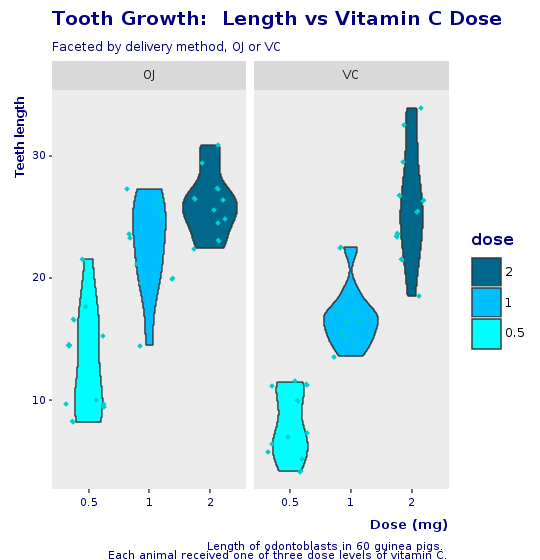
\includegraphics[width=0.70000\textwidth]{figures/final_violin_plot.png}
\caption{}
\end{figure}

\subsection{Another View}\label{another-view}

Finally, here is a last plot, with the same look and feel as before but
facetted by dose and not by supplement.

\begin{Shaded}
\begin{Highlighting}[]
\NormalTok{R.png(}\StringTok{"figures/facet_by_dose.png"}\NormalTok{, }\StringTok{width: }\DecValTok{540}\NormalTok{, }\StringTok{height: }\DecValTok{560}\NormalTok{)}

\NormalTok{caption = <<-}\KeywordTok{EOT}
\OtherTok{Length of odontoblasts in 60 guinea pigs. }
\OtherTok{Each animal received one of three dose levels of vitamin C.}
\KeywordTok{EOT}

\OtherTok{@bp}\NormalTok{ = }\OtherTok{@tooth_growth}\NormalTok{.ggplot(E.aes(}\StringTok{x: :supp}\NormalTok{, }\StringTok{y: :len}\NormalTok{, }\StringTok{group: :supp}\NormalTok{)) + }
\NormalTok{      R.geom_boxplot(E.aes(}\StringTok{fill: :supp}\NormalTok{)) + R.facet_grid(+}\StringTok{:all}\NormalTok{ =~ +}\StringTok{:dose}\NormalTok{) +}
\NormalTok{      R.scale_fill_manual(}\StringTok{values: }\NormalTok{R.c(}\StringTok{"cyan"}\NormalTok{, }\StringTok{"deepskyblue4"}\NormalTok{)) +}
\NormalTok{      R.labs(}\StringTok{title: "Tooth Growth:  Length by Dose"}\NormalTok{,}
             \StringTok{subtitle: "Faceted by dose"}\NormalTok{,}
             \StringTok{x: "Delivery method"}\NormalTok{, }\StringTok{y: "Teeth length"}\NormalTok{,}
             \StringTok{caption: }\NormalTok{caption) +}
      \DataTypeTok{CorpTheme}\NormalTok{.global_theme(}\StringTok{faceted: }\DecValTok{true}\NormalTok{)}
\NormalTok{puts }\OtherTok{@bp}

\NormalTok{R.dev__off}
\end{Highlighting}
\end{Shaded}

\begin{figure}
\centering
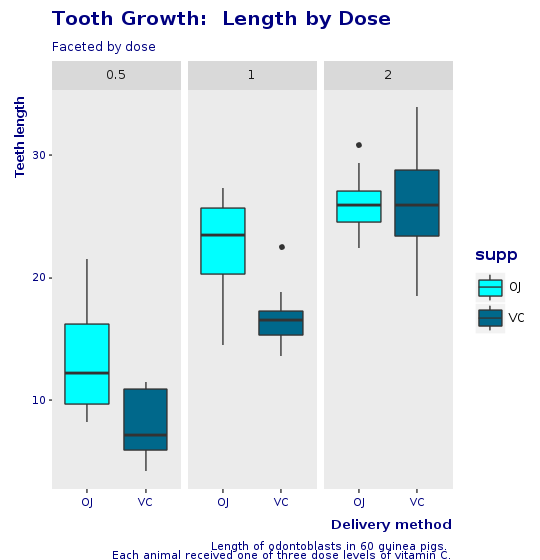
\includegraphics[width=0.70000\textwidth]{figures/facet_by_dose.png}
\caption{}
\end{figure}

\section{Conclusion}\label{conclusion}

Galaaz tightly couples Ruby and R in a way that Ruby developers do not
need to be aware of the executing R engine. For the Ruby developer the
existence of R is of no consequence. For her, she is just coding in
Ruby. On the other hand, for the R developer, migration to Ruby is a
matter of small syntactic changes and very gentle learning curve. As the
R developer becomes more proficient in Ruby, he can start using
`classes', `modules', `procs', `lambdas'.

This coupling shows the power of GraalVM and Truffle polyglot
environment. Trying to bring to Ruby the power of R starting from
scratch is an enourmous endeavour and would probably never be
accomplished. Today's data scientists would certainly stick with either
Python or R. Now, both the Ruby and R communities might benefit from
this marriage. Also, the process to couple Ruby and R can be also be
done to couple Ruby and JavaScript and maybe also Ruby and Python. In a
polyglot world a \emph{uniglot} language might be extremely relevant.

From the perspective of performance, GraalVM and Truffle promises
improvements that could reach over 10 times, both for
\href{https://medium.com/graalvm/faster-r-with-fastr-4b8db0e0dceb}{FastR}
and for
\href{https://rubykaigi.org/2018/presentations/eregontp.html}{TruffleRuby}.

This article has shown how to improve a plot step-by-step. Starting from
a very simple boxplot with all default configurations, we moved slowly
to our final plot. The important point here is not if the final plot is
actually beautiful, but that there is a process of small steps
improvements that can be followed until getting a final plot ready for
presentation.

Finally, this whole article was written in rmarkdown and compiled to
HTML by \emph{gknit}, an application that wraps \emph{knitr} and allows
documenting Ruby code. This application can be of great help for any
Rubyist trying to write articles, blogs or documentation for Ruby.

\section{Installing Galaaz}\label{installing-galaaz}

\subsection{Prerequisites}\label{prerequisites}

\begin{itemize}
\tightlist
\item
  GraalVM (\textgreater{}= rc8):
  \url{https://github.com/oracle/graal/releases}
\item
  TruffleRuby
\item
  FastR
\end{itemize}

The following R packages will be automatically installed when necessary,
but could be installed prior to using gKnit if desired:

\begin{itemize}
\tightlist
\item
  ggplot2
\item
  gridExtra
\item
  knitr
\end{itemize}

Installation of R packages requires a development environment and can be
time consuming. In Linux, the gnu compiler and tools should be enough. I
am not sure what is needed on the Mac.

\subsection{Preparation}\label{preparation}

\begin{itemize}
\tightlist
\item
  gem install galaaz
\end{itemize}

\subsection{Usage}\label{usage}

\begin{itemize}
\tightlist
\item
  gknit 
\item
  In a scrip add: require `galaaz'
\end{itemize}


\end{document}
